\chapter{Marco teórico}

En los últimos años, el uso de la Inteligencia Artificial (IA) se ha disparado, especialmente a partir de la aparición de ChatGPT en noviembre de 2022. A menudo se habla de la IA como si hubiese surgido en ese momento, pero en realidad lleva mucho más tiempo existiendo. Lo que se popularizó en 2022 es una rama concreta de la Inteligencia Artificial: la IA generativa, que en apenas tres años ha acaparado gran parte de la atención pública y mediática, eclipsando otras disciplinas dentro del campo. Con el tiempo se ha generalizado el término \textit{IA} popularmente, sustituyendo al término IA generativa.

La IA es un área de la informática y las matemáticas que busca desarrollar sistemas capaces de realizar tareas que normalmente requieren inteligencia humana, como el razonamiento, el aprendizaje o la comprensión del lenguaje. Sus orígenes se sitúan en los años cincuenta, con el célebre test de Turing, para detectar si algo es una máquina o un humano, y el Dartmouth Workshop de 1956, considerado el nacimiento oficial de la disciplina \cite{McCarthy1956Dartmouth}. En las décadas siguientes se desarrollaron los primeros algoritmos de búsqueda y decisión, como Minimax y A*, que representan la llamada IA simbólica, basada en reglas, lógica y búsqueda sistemática. 

A partir de los años noventa, el Aprendizaje Automático (Machine Learning, ML) marcó un cambio de paradigma, seguido por el auge del Aprendizaje Profundo (Deep Learning, DL) en la década de 2010 gracias al uso de redes neuronales profundas. Estas disciplinas se organizan de manera jerárquica, como se puede ver en la Figura \ref{fig:ia-ml-dl-gen}. Finalmente, desde 2018 en adelante, la IA generativa y los modelos de lenguaje de gran tamaño (Large Language Models, LLM) han transformado el panorama, permitiendo aplicaciones como ChatGPT y consolidando la IA como un fenómeno global.

\begin{figure}[H]
    \centering
    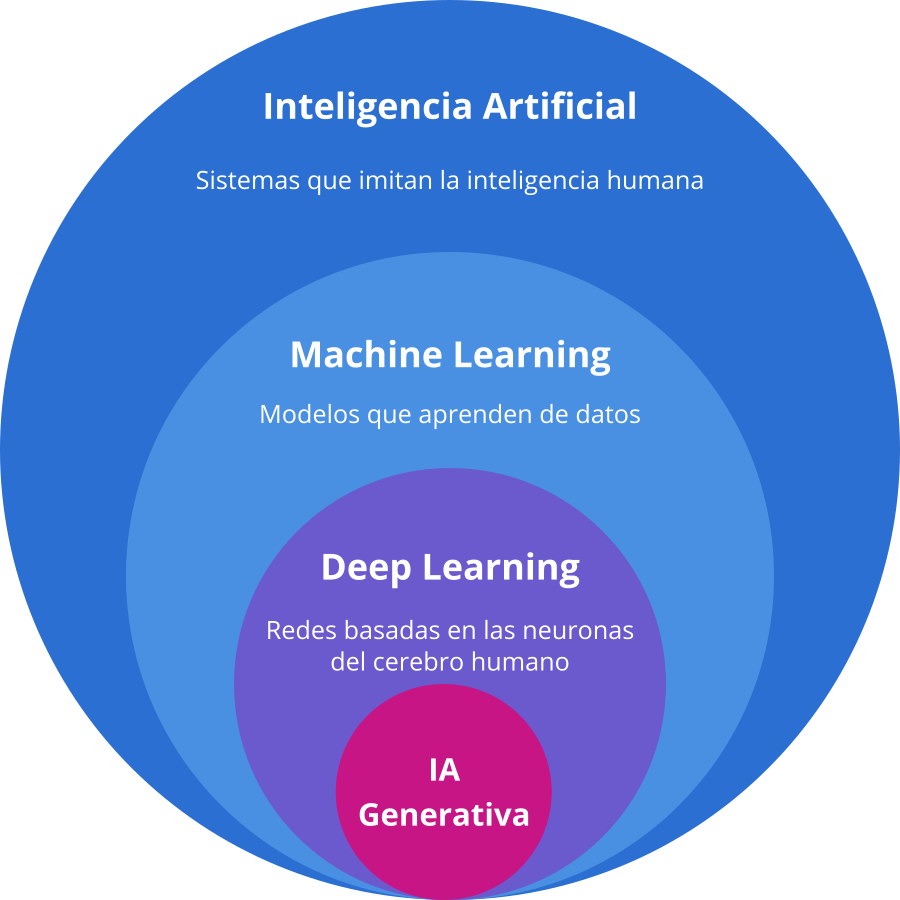
\includegraphics[width=0.6\textwidth]{figures/ia_jerarquica.png}    
    \caption{\label{fig:ia-ml-dl-gen} Relación entre IA, ML, DL e IA generativa. De creación propia.}
\end{figure}


Este TFG se centra en el Aprendizaje Profundo y el PLN, áreas dentro del Aprendizaje Automático, que como como su propio nombre indica, consisten en que el modelo \textit{aprende}, infiriendo conclusiones de datos que se le muestran. El Deep Learning se basa en el uso de redes neuronales artificiales para aprender patrones y relaciones complejas.

\section{Aprendizaje profundo y redes neuronales}
\label{redes-neuronales}

Las \textbf{redes neuronales artificiales} son algoritmos inspirados en el comportamiento de las neuronas humanas. Cada neurona artificial realiza una operación similar a una regresión lineal, combinando las entradas mediante una suma ponderada y añadiendo un \textit{sesgo}. Sin embargo, una combinación de regresiones lineales sigue siendo equivalente a otra regresión lineal, por lo que se introducen funciones de activación no lineales —como la sigmoide o la ReLU— que permiten a la red modelar relaciones más complejas.

Para entrenar estas redes se utiliza el algoritmo de \textbf{retropropagación del gradiente (backpropagation)}. Este método calcula el error de salida de la red y lo propaga hacia atrás capa por capa, ajustando los pesos mediante descenso del gradiente. En cada iteración, los parámetros se modifican en la dirección que minimiza la función de pérdida, permitiendo que la red aprenda progresivamente a realizar la tarea deseada.


\section{Arquitectura Transformer}
\label{transformers}

\subsection{Arquitectura general del Transformer}

Las arquitecturas previas de redes neuronales presentaban limitaciones a la hora de generar texto coherente y de manejar dependencias largas dentro de una secuencia. Para superar estos problemas, en 2017 se presentó la arquitectura \textbf{Transformer}, descrita en el artículo \textit{Attention is All You Need} \cite{vaswani2023attentionneed}. Esta arquitectura introdujo un cambio fundamental en el procesamiento del lenguaje natural.

El Transformer está organizado en dos bloques principales:

\begin{itemize}
    \item \textbf{Encoder}: procesa la secuencia de entrada y genera representaciones contextuales.
    \item \textbf{Decoder}: genera la salida token a token, utilizando tanto la información previa generada como la del encoder.
\end{itemize}

Cada bloque está compuesto por varias capas que combinan tres elementos fundamentales:

\begin{itemize}
    \item \textbf{Capas de atención}, que permiten al modelo identificar qué partes de la secuencia son relevantes en cada momento.
    \item \textbf{Capas de normalización}, que estabilizan el entrenamiento y evitan problemas en la retropropagación.
    \item \textbf{Capas \textit{Feed Forward}}, que son redes neuronales aplicadas de manera independiente a cada token (véase Sección \ref{redes-neuronales}).
\end{itemize}

En la Figura \ref{fig:estructura-transformers} se muestra la arquitectura original propuesta en \cite{vaswani2023attentionneed}.

\begin{figure}[H]
    \centering
    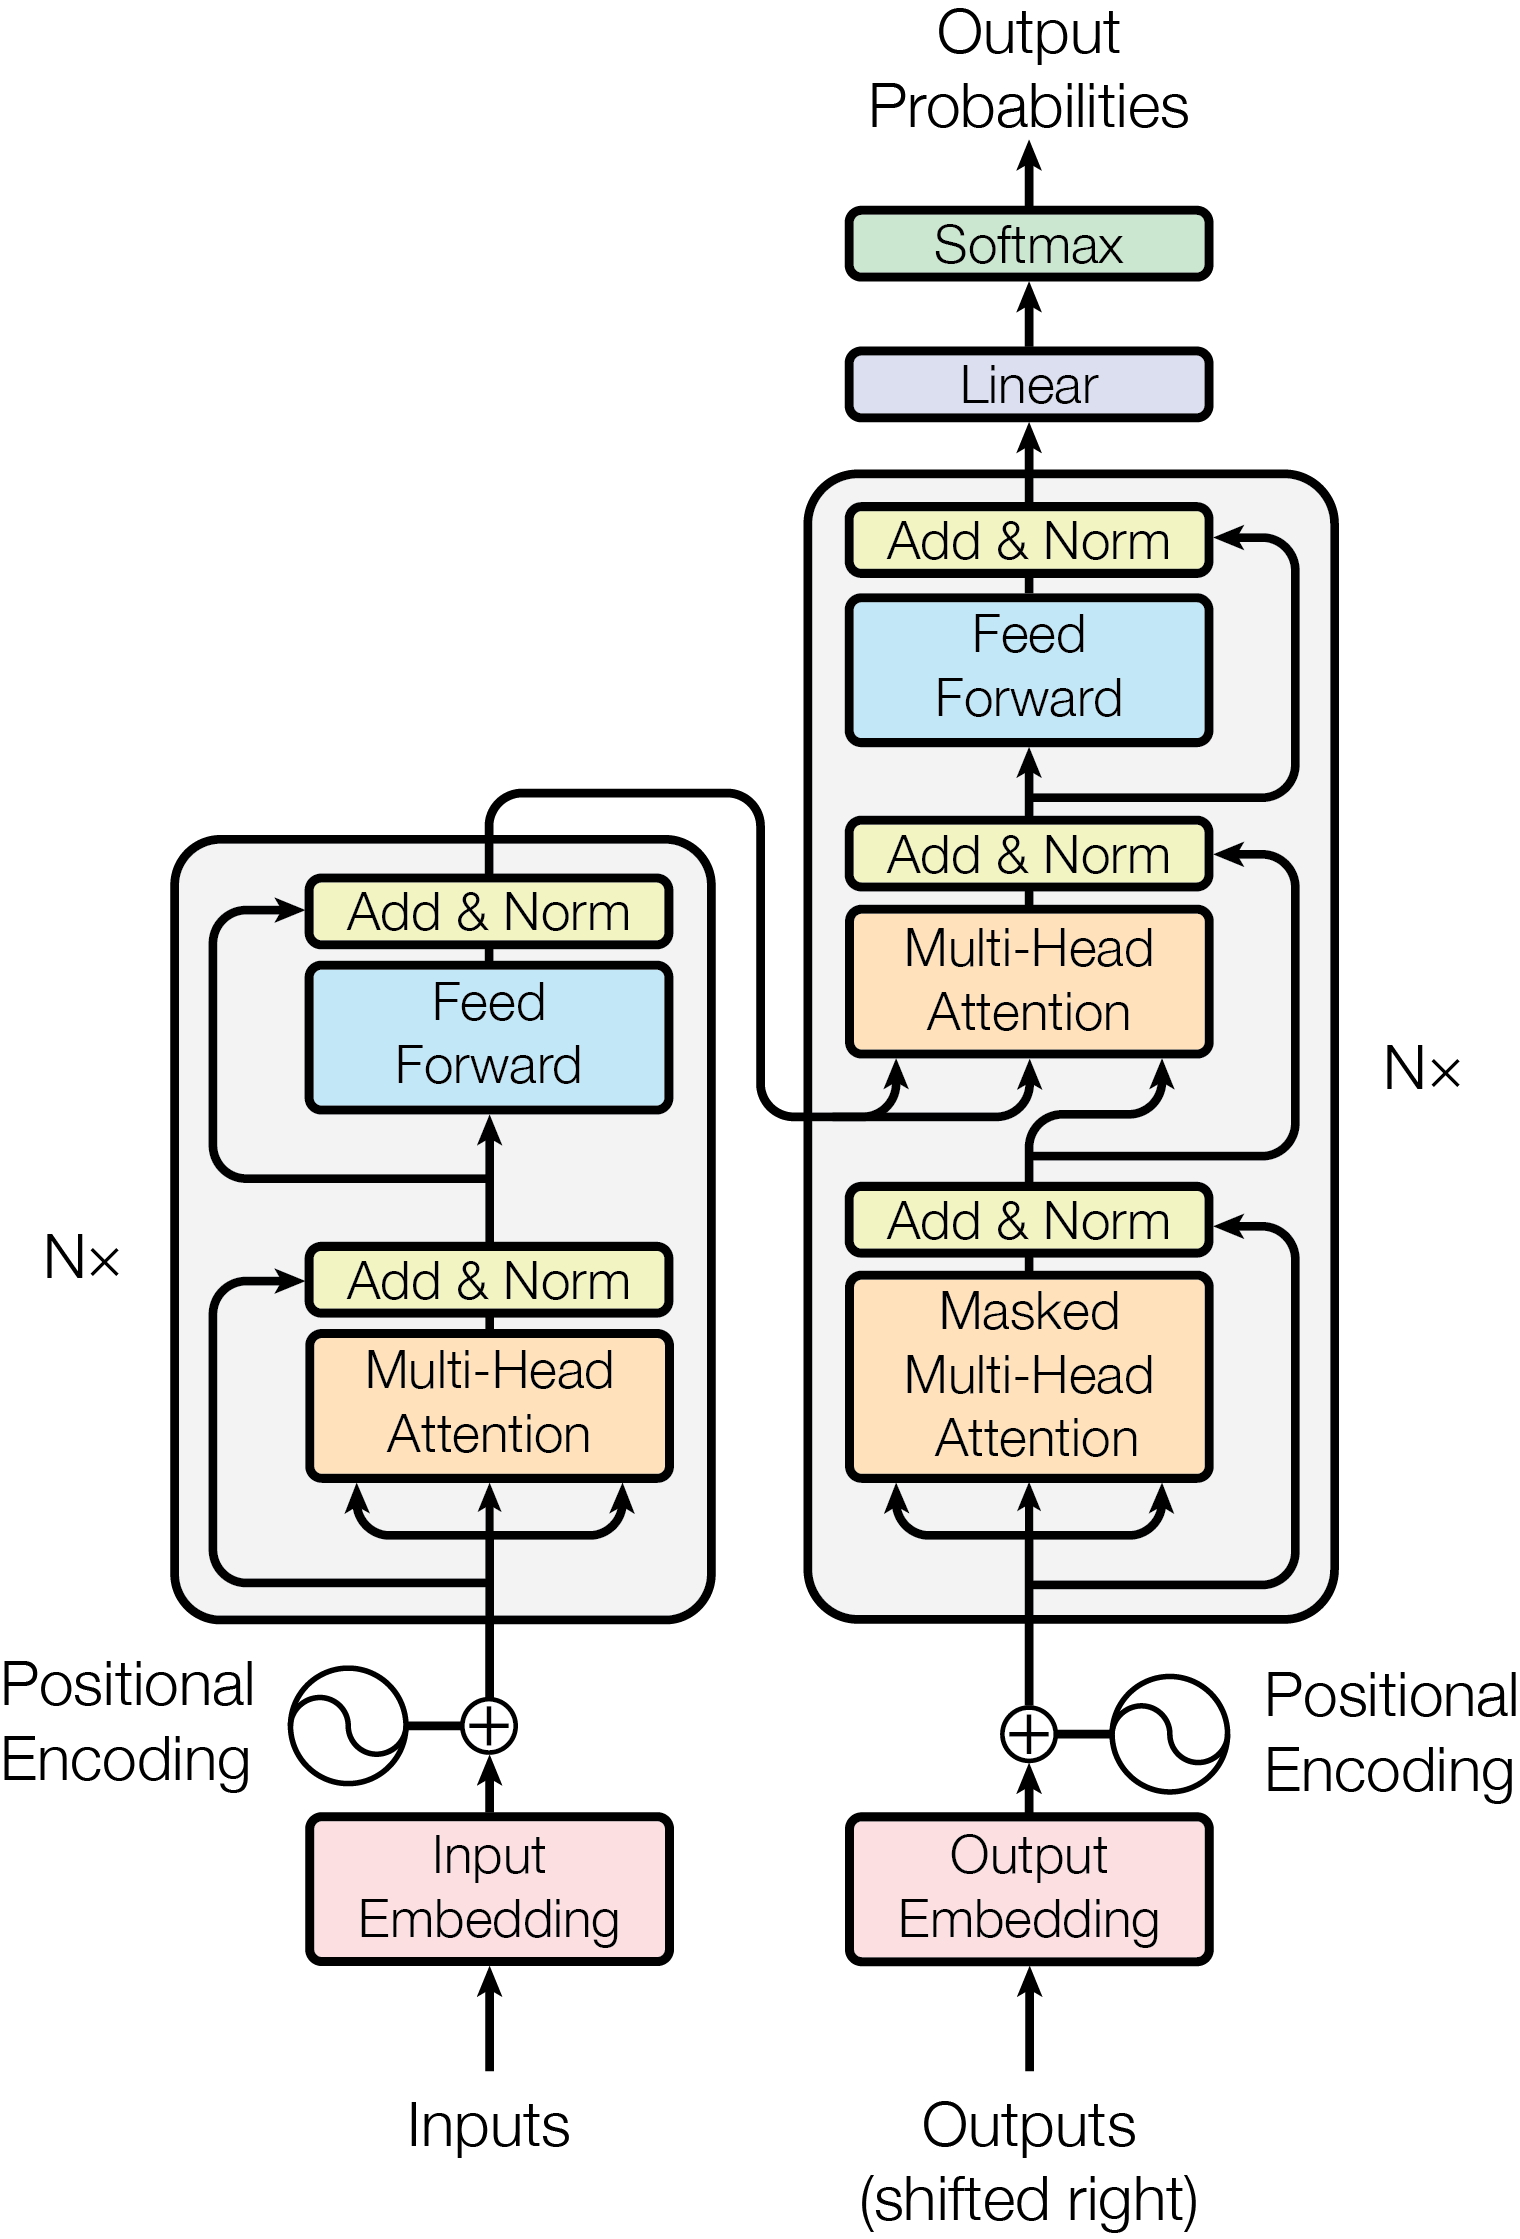
\includegraphics[width=0.5\textwidth]{figures/AttentionIsAllYouNeed.png}    
    \caption{\label{fig:estructura-transformers} Esquema de la arquitectura de un transformer \cite{vaswani2023attentionneed}.}
\end{figure}


\subsection{El mecanismo de atención}

El componente más innovador del Transformer es el mecanismo de \textbf{atención}. Este mecanismo permite procesar secuencias completas en paralelo y determinar qué partes de la entrada son más relevantes en cada contexto, algo que las arquitecturas anteriores no podían hacer de manera eficiente. La idea central es que cada token de la secuencia pueda “mirar” al resto de tokens y decidir, mediante un cálculo numérico, cuáles contienen información útil para interpretar su significado.

Para ello utiliza tres matrices fundamentales: \textbf{Query (Q)}, \textbf{Key (K)} y \textbf{Value (V)}. Cada token se proyecta en estas tres representaciones, y el modelo compara las Query con las Key para obtener una medida de similitud. Cuanto mayor es esta similitud, mayor es la atención que se asigna al token correspondiente. Esa atención se utiliza después para combinar las Value y generar una representación contextualizada, que ya no depende únicamente del token aislado, sino de su relación con el resto de la secuencia.

Este proceso permite capturar dependencias largas, como referencias a palabras que aparecen muchas posiciones antes, y también relaciones más sutiles, como concordancias gramaticales o estructuras sintácticas complejas. Además, el Transformer no se limita a una única atención, sino que utiliza varias en paralelo, conocidas como \textit{multi-head attention}. Cada cabeza aprende a fijarse en un tipo distinto de relación. Algunas detectan estructura sintáctica, otras relaciones semánticas y otras patrones más abstractos. La combinación de todas ellas produce una representación rica y expresiva del texto.

Gracias a este mecanismo, el modelo puede comprender mejor el contexto global de la secuencia y generar representaciones mucho más precisas que las obtenidas con arquitecturas recurrentes o convolucionales. La atención es, por tanto, el núcleo que permite a los Transformers escalar a grandes cantidades de datos y alcanzar el rendimiento que caracteriza a los modelos actuales.


\subsection{Inferencia y generación de texto}

El proceso de generación en un Transformer se realiza \textbf{token a token}. La salida del modelo es un vector del tamaño del vocabulario, donde cada posición representa la probabilidad de que ese token sea el siguiente. Para generar secuencias más largas, se calcula la probabilidad del siguiente token. Después se selecciona el token más probable (añadiendo aleatoriedad, para que el modelo suene más natural, llamada temperatura) y ese token se reintroduce al final del texto anterior como entrada del modelo. El proceso se repite hasta alcanzar la longitud deseada o un token de parada.

Este procedimiento permite generar texto coherente y contextualizado, aunque también introduce desafíos como la acumulación de errores o la pérdida de coherencia en secuencias largas.


\subsection{Variantes del Transformer}

El Transformer puede utilizarse de distintas maneras, dependiendo de los bloques que se utilicen:

\begin{itemize}
    \item \textbf{Encoder–Decoder} \cite{vaswani2023attentionneed}: Cogiendo el transformer completo, utilizado en tareas como la traducción automática.
    \item \textbf{Solo Encoder} \cite{devlin2019bert}: Genera representaciones semánticas numéricas de textos (por ejemplo, BERT).
    \item \textbf{Solo Decoder} \cite{brown2020language}: Arquitectura más utilizada para generación de texto, empleada por modelos como GPT, LLaMA o Qwen.
\end{itemize}

Los modelos utilizados en este proyecto pertenecen a esta última categoría, ya que están diseñados específicamente para la generación de texto.

\subsection{Impacto en los modelos de lenguaje}

La introducción de esta arquitectura supuso un salto cualitativo en tareas como la generación de texto, la traducción automática y el procesamiento del lenguaje natural en general. Gracias a los Transformers fue posible desarrollar modelos cada vez más grandes y sofisticados, dando lugar a los actuales \textbf{modelos de lenguaje de gran tamaño (LLM)}, capaces de producir resultados de alta calidad en aplicaciones como ChatGPT \cite{vaswani2023attentionneed}.


\section{Modelos de Lenguaje de Gran Tamaño (Large Language Models, LLM)}

Los LLM son arquitecturas basadas en los Transformers que, entrenadas con enormes cantidades de datos, pueden generar y comprender texto, imágenes o sonido. Entre los LLM más conocidos actualmente se encuentran GPT de OpenAI, Gemini de Google o DeepSeek, de código abierto. Estos modelos presentan varios problemas, como los sesgos derivados de los datos con los que fueron entrenados y que, en consecuencia, pueden reproducir. Además, sufren de alucinaciones, es decir, generan información inventada o sin fundamento. Sin embargo, el problema en el que se enfoca este trabajo es otro. Al necesitar grandes cantidades de datos para ser entrenados, los modelos aprenden principalmente de lenguas con abundantes recursos disponibles en internet. La principal lengua con la que se han entrenado es el inglés, lo que genera desigualdad y deja en riesgo de invisibilización a las lenguas minoritarias.

\section{Fine tuning eficiente en LLM}

Entrenar un LLM desde cero es una tarea que muy pocas instituciones o empresas pueden realizar, ya que requiere un cómputo extremadamente alto. Por eso, este trabajo se basa en una estrategia común para mejorar el rendimiento de los LLM, en vez de reentrenarlos completamente, se utiliza la técnica de \textbf{Ajuste Eficiente de Parámetros (Parameter Efficient Fine Tuning, PEFT)}. La técnica de PEFT más utilizada es \textbf{Low-Rank Adaptation (LoRA)}. La idea de LoRA consiste en añadir al peso original, de ciertas capas del transformer, una modificación entrenable de bajo rango \cite{gang:hal-04983079}. Suponiendo que una capa de la red tiene una matriz de pesos de tamaño \(N \times M\), con \(N \cdot M\) parámetros. En lugar de ajustar todos ellos, LoRA introduce dos matrices de rango reducido: 



\[
A \in \mathbb{R}^{N \times r}, \quad B \in \mathbb{R}^{r \times M}
\]



de tal manera que su producto \(A \cdot B\) genera una actualización de tamaño \(N \times M\). El número de parámetros entrenables pasa de \(N \cdot M\) a \(r \cdot (N + M)\), lo que supone un ahorro muy significativo.

Por ejemplo, si una capa tiene una matriz de pesos de tamaño \(4096 \times 4096\), el número de parámetros originales es:



\[
4096 \cdot 4096 = 16{.}777{,}216
\]



Si aplicamos LoRA con un rango reducido \(r = 8\), las dos matrices entrenables tienen:



\[
4096 \cdot 8 + 8 \cdot 4096 = 65{,}536
\]



Esto significa que en lugar de entrenar más de 16 millones de parámetros, solo se entrenarían unos 65 mil, lo que supone un ahorro superior al 99.6\% de los valores. Gracias a esta reducción, LoRA permite adaptar modelos muy grandes a nuevas tareas o lenguas con recursos limitados de manera práctica y eficiente.

Además de LoRA, en los últimos años ha surgido una variante especialmente útil en contextos con recursos limitados, \textbf{QLoRA}. Esta técnica combina las ventajas de LoRA con una cuantización del modelo base a 4 bits, lo que reduce drásticamente el uso de memoria sin afectar al rendimiento. QLoRA alcanza resultados equivalentes a los de LoRA tradicional incluso en modelos de gran tamaño, permitiendo realizar \textit{fine-tuning} eficiente en hardware modesto \cite{dettmers2023qlora}. Gracias a esta reducción de requisitos computacionales y a su estabilidad, QLoRA se ha convertido en una de las opciones más adecuadas para adaptar LLMs a nuevas lenguas.

